\documentclass[11pt]{article}

\usepackage[margin=1in]{geometry}
\usepackage{amsmath}
\usepackage{booktabs}
\usepackage{graphicx}
\usepackage{float}
\usepackage{placeins}
\usepackage{hyperref}

\graphicspath{{../docs/}}
\hypersetup{colorlinks=true, linkcolor=blue, urlcolor=blue}

\title{FRB/US Macroeconomic Model in Dynare}
\author{Technical draft}
\date{July 2026}

\begin{document}
\maketitle

\begin{abstract}
This report describes a Dynare implementation of the Federal Reserve FRB/US
macroeconomic model translated from BIMETS model-definition language (MDL).
The repository contains a backward-looking version and a model-consistent
expectations (MCE) version. The implementation is a path-simulation
replication: historical data determine equation-specific tracking residuals,
and Dynare's nonlinear perfect-foresight solver evaluates counterfactual
paths. Four exercises demonstrate a monetary-policy shock, the corresponding
MCE experiment, propagation of model residuals, and endogenous targeting. A
stochastic bootstrap is included as an optional extension.
\end{abstract}

\tableofcontents
\newpage

\section{Purpose and scope}

FRB/US is a large-scale quarterly macroeconomic model. The goal of this
repository is to make a reproducible Dynare path-simulation version of the
public BIMETS representation. The implementation does not estimate
parameters, construct a posterior distribution, or replace the source model's
equations with a small textbook model. Instead, it preserves the translated
equations and uses the observed LONGBASE path to recover the add-factors that
make the model reproduce the baseline.

The workflow is useful for studying the mechanics of FRB/US counterfactuals:
the baseline is first reconstructed, then one or more add-factors or policy
paths are modified, and the nonlinear system is solved again. This separation
also makes numerical errors distinguishable from differences in scenario
definition.

\section{Source model and translation}

The source files are \texttt{source/frbus\_model.txt} for the
backward-looking model and \texttt{source/frbus\_model\_mce.txt} for the MCE
model. The Python converter in
\texttt{scripts/parse\_frbus\_mdl.py} parses the MDL identity blocks, converts
time operators to Dynare timing, writes the equation includes, and generates
MATLAB functions for add-factor construction.

Both versions contain 284 unique endogenous variables, 293 identity blocks,
and 83 listed exogenous variables. The MCE version replaces selected
expectation relationships with forward-looking equations and has a maximum
lead of eight quarters in the source inventory.

The main operator translations are:

\begin{table}[H]
\centering
\caption{Selected MDL to Dynare translations.}
\begin{tabular}{ll}
\toprule
MDL operator & Dynare form \\
\midrule
\texttt{TSLAG(x,n)} & \texttt{x(-n)} \\
\texttt{TSLEAD(x,n)} & \texttt{x(+n)} \\
\texttt{TSDELTA(x)} & \texttt{x - x(-1)} \\
\texttt{TSDELTALOG(x)} & \texttt{log(x) - log(x(-1))} \\
\texttt{MOVAVG(x,n)} & \texttt{(x + x(-1) + ... + x(-(n-1)))/n} \\
\texttt{LOG(x)}, \texttt{EXP(x)} & \texttt{log(x)}, \texttt{exp(x)} \\
\bottomrule
\end{tabular}
\end{table}

The seven conditional blocks in the source are retained as exact \texttt{max()}
relationships. This keeps the economic thresholds visible and avoids silently
changing the model near a kink.

\section{Tracking residuals and baseline replication}

For each endogenous variable $y$, the translated equation is written as

\begin{equation}
y_t = f_y(\text{current, lagged, and lead variables};\ \text{exogenous inputs}) + a_{y,t}.
\end{equation}

Here $a_{y,t}$ is an equation-specific tracking residual. Given a data path,
the add-factor function evaluates

\begin{equation}
a_{y,t} = y_t^{\text{data}} - f_y(\text{data path at }t).
\end{equation}

The baseline solver initializes Dynare's original and auxiliary lag/lead
variables from the same data path. This matters because zero-filled
auxiliary histories can create an artificial first-period discrepancy even
when the add-factor identity is correct.

The bundled CSV is a row-index-only LONGBASE export with 848 quarterly rows.
The loader maps row 1 to 1962Q1 and reconstructs quarter labels through
2173Q4. An external file with a date column is read from its own dates; an
external row-index-only file can supply a different starting quarter.

The v4 validation window for the backward model is 2040Q1--2045Q4. With
\texttt{dfpdbt = 0} and \texttt{dfpsrp = 1}, the no-shock solution has

\begin{center}
\begin{tabular}{lr}
\toprule
Statistic & Value \\
\midrule
Maximum absolute error & $9.50\times 10^{-9}$ \\
Mean absolute error & $4.17\times 10^{-11}$ \\
\bottomrule
\end{tabular}
\end{center}

These errors are numerical solver tolerances rather than a re-estimation of
the model.

\section{Dynare solution workflow}

The `.mod` files declare the original endogenous and exogenous variables plus
one add-factor for each endogenous equation. The source equations are
included with the Dynare preprocessor. Scenario scripts then:

\begin{enumerate}
\item load LONGBASE-compatible data and map it to quarterly IDs;
\item set policy switches and compute baseline add-factors;
\item initialize a finite perfect-foresight window;
\item apply the scenario change to add-factors or target paths;
\item solve the nonlinear system with Dynare; and
\item export tables and pyfrbus-style charts.
\end{enumerate}

The MCE example requires terminal values because of forward-looking equations.
The demonstration therefore reports a short early window; a longer terminal
horizon is preferable for research applications.

\section{Exercise 1: backward-looking monetary-policy shock}

The first exercise applies a 100 basis point shock to the add-factor of
\texttt{rffintay} in 2040Q1. The simulation runs through 2045Q4 with
\texttt{dfpdbt = 0} and \texttt{dfpsrp = 1}. The headline panels show GDP
growth and core PCE inflation as four-quarter percent changes computed from
\texttt{xgdp} and \texttt{pcxfe}; unemployment and the federal funds rate are
shown in levels. The chart includes pre-shock history to make the transition
visible.

\begin{figure}[H]
\centering
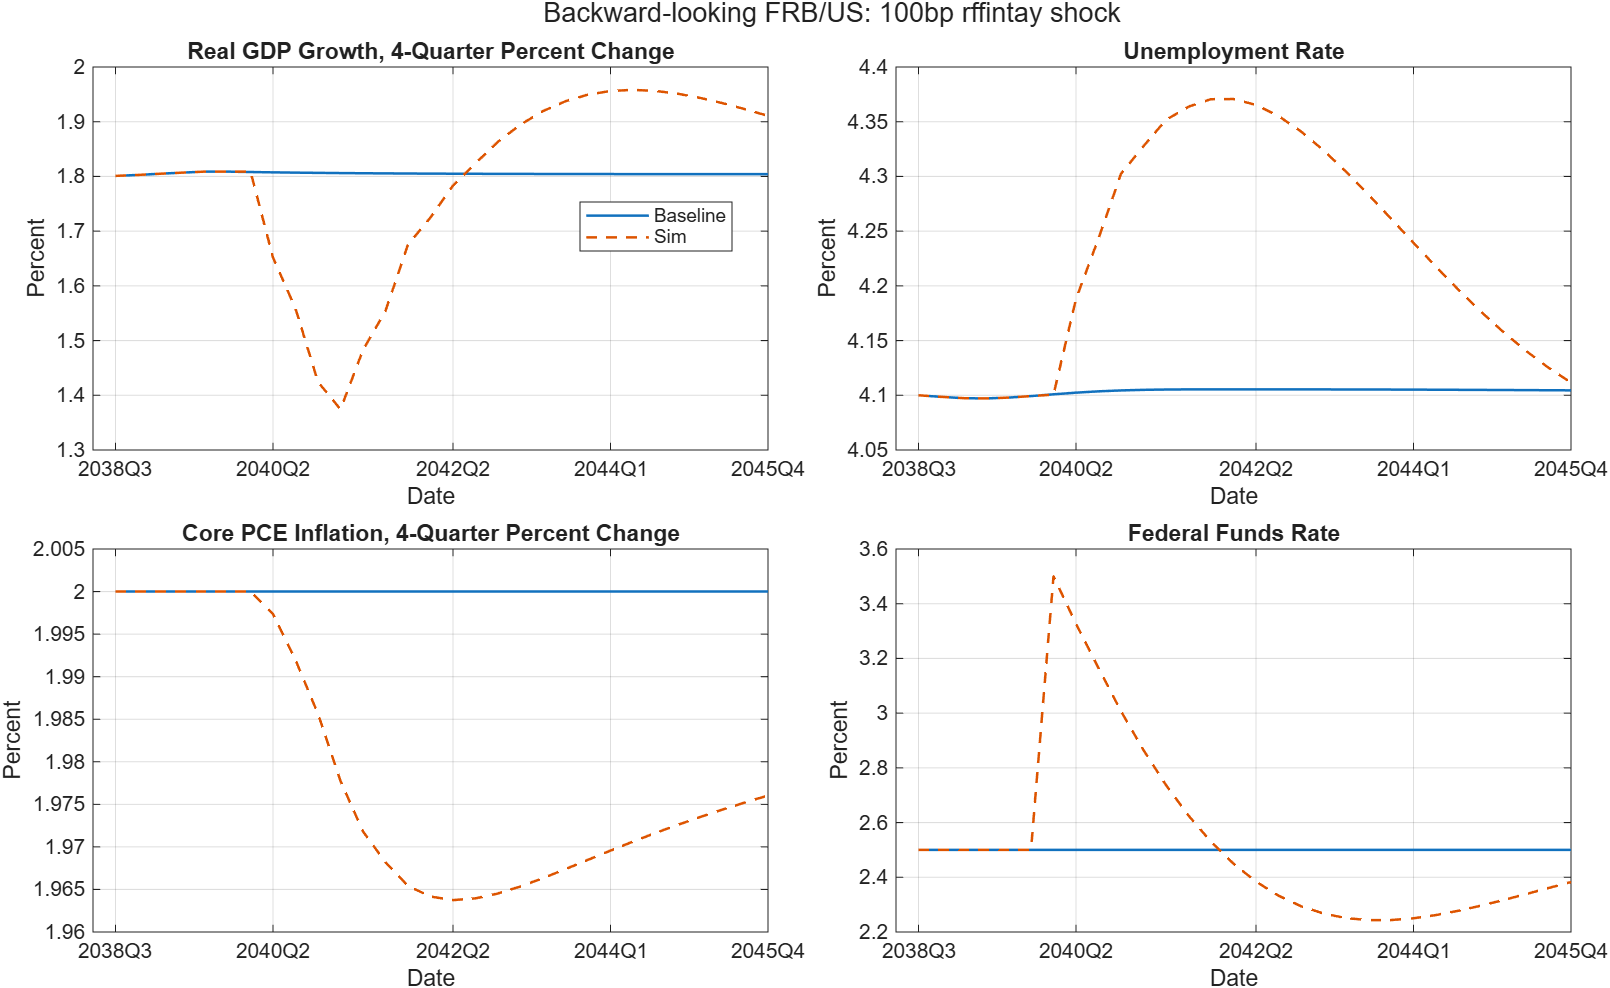
\includegraphics[width=0.94\linewidth]{mp_shock_backward_pyfrbus_style.png}
\caption{Backward-looking model: 100 bp monetary-policy shock.}
\label{fig:mpbackward}
\end{figure}
\FloatBarrier

The expected qualitative response is an immediate rise in the federal funds
rate, followed by weaker activity, higher unemployment with a lag, and a
gradual decline in core inflation. The complete path table is written to
\texttt{docs/mp\_shock\_backward\_paths.csv}.

\section{Exercise 2: model-consistent expectations shock}

The second exercise applies the same policy shock to the MCE representation.
It uses 2040Q1--2041Q4, sets \texttt{drstar = 0} initially, and turns
\texttt{drstar} on from 2041Q1. The shorter window is a demonstration of the
forward-looking model and its terminal-value requirement, not a restriction
on longer research simulations.

\begin{figure}[H]
\centering
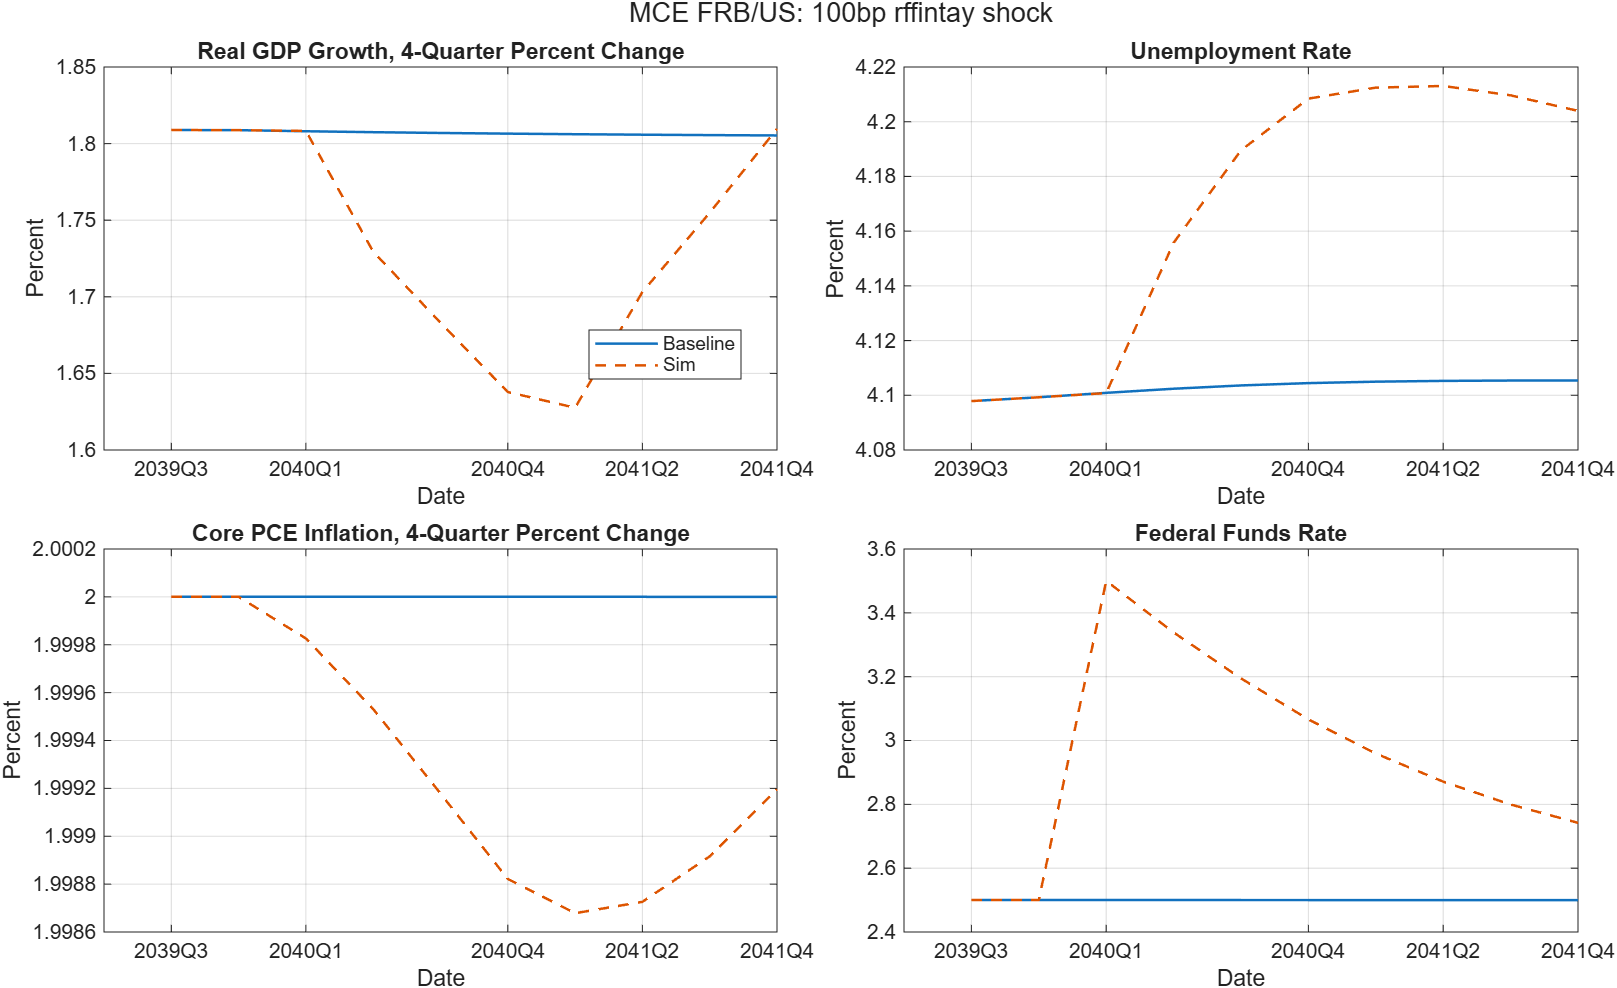
\includegraphics[width=0.94\linewidth]{mp_shock_mce_pyfrbus_style.png}
\caption{MCE model: short-horizon 100 bp monetary-policy shock.}
\label{fig:mce}
\end{figure}
\FloatBarrier

The first reported quarter is close to the backward-looking result, while
the forward-looking equations affect the subsequent path. The MCE path table
is written to \texttt{docs/mp\_shock\_mce\_paths.csv}.

\section{Exercise 3: error propagation}

The third exercise starts with baseline tracking residuals, preserves the
policy configuration, and applies a persistent residual shock. The shock is
ramped into the model through continuation steps so that the nonlinear solver
starts each step from the previous converged path. This is numerically useful
for a large system with threshold equations and does not alter the final
scenario definition.

\begin{figure}[H]
\centering
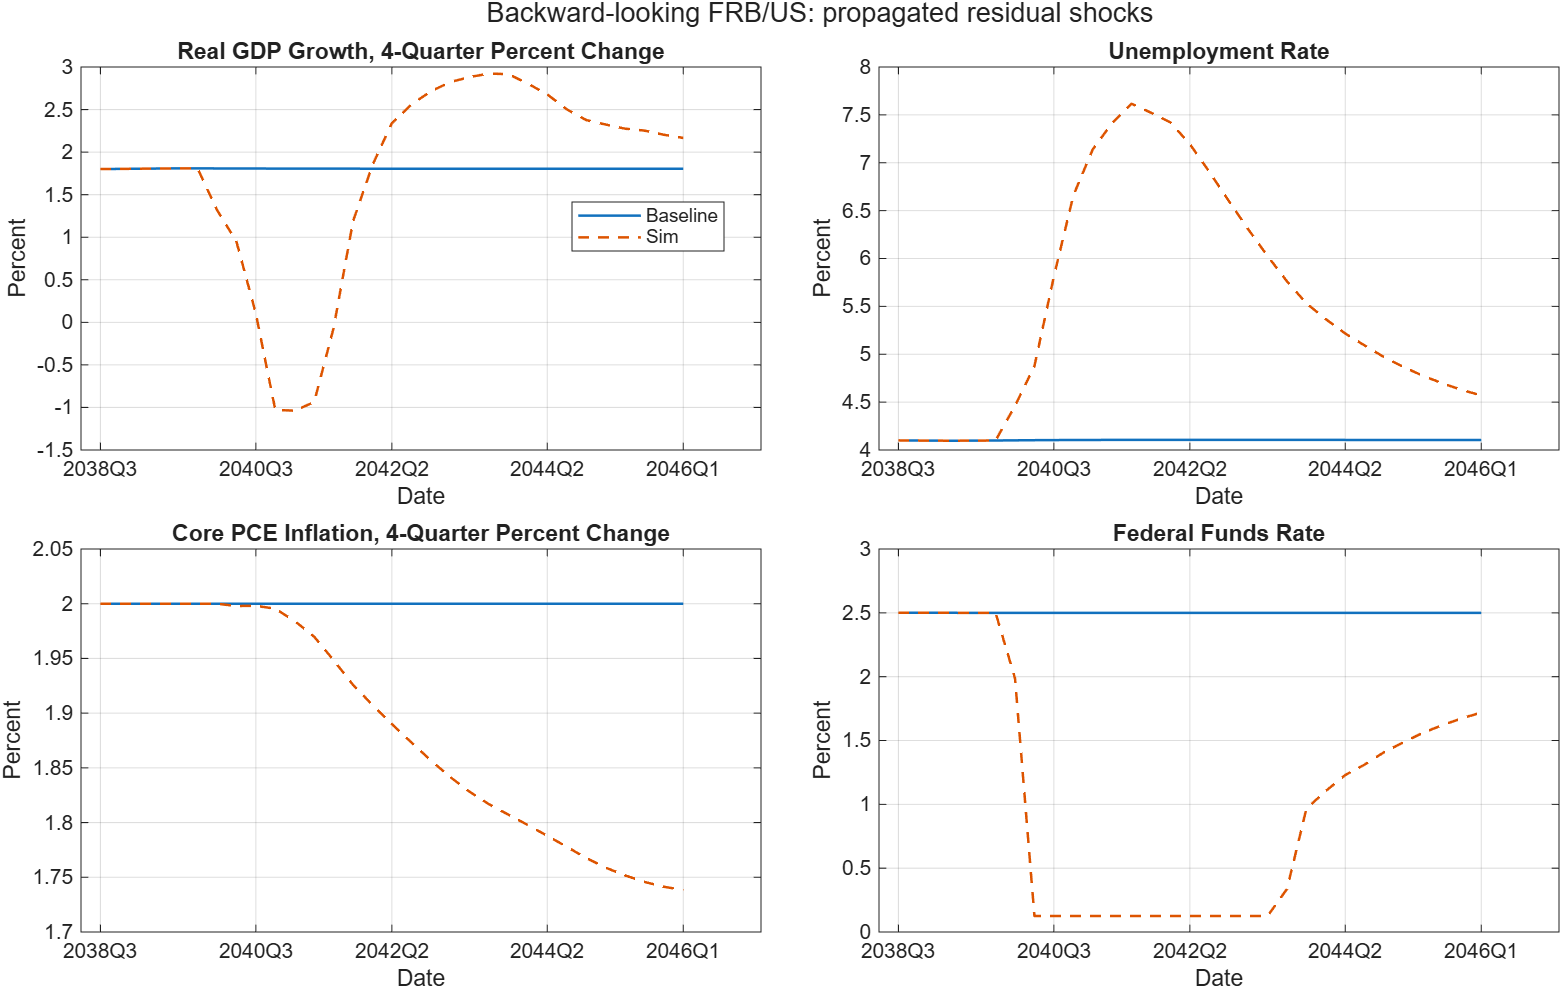
\includegraphics[width=0.94\linewidth]{error_propagation_backward_pyfrbus_style.png}
\caption{Backward-looking model: propagated residual shock.}
\label{fig:errorprop}
\end{figure}
\FloatBarrier

The output table is \texttt{docs/error\_propagation\_backward\_paths.csv}.
The scenario script also checks the solver status at every continuation step
before writing the final chart.

\section{Exercise 4: endogenous targeting}

The fourth exercise implements a transparent external Newton controller. It
adjusts five add-factor instruments, \texttt{eco}, \texttt{lhp},
\texttt{picxfe}, \texttt{rff}, and \texttt{rg10p}, to match five target paths
for \texttt{xgdp}, \texttt{lur}, \texttt{picxfe}, \texttt{rff}, and
\texttt{rg10} from 2021Q3 through 2022Q3. The controller uses finite
differences, damping through a maximum step, and repeated perfect-foresight
solves.

\begin{figure}[H]
\centering
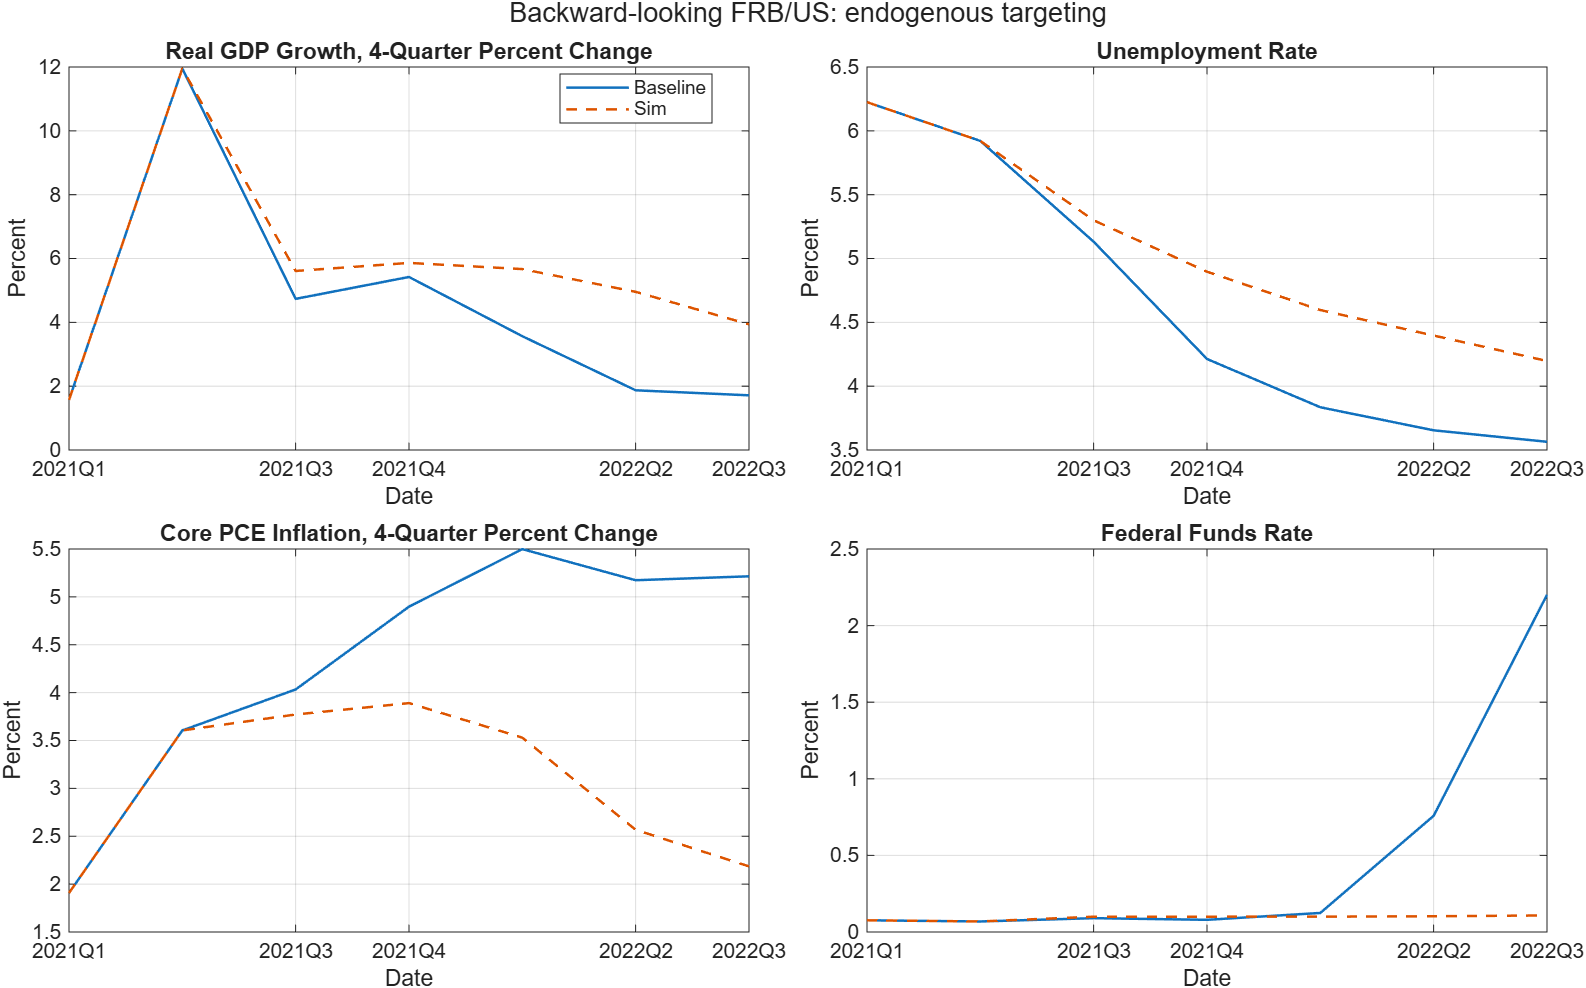
\includegraphics[width=0.94\linewidth]{endogenous_targeting_backward_pyfrbus_style.png}
\caption{Backward-looking model: endogenous targeting exercise.}
\label{fig:targeting}
\end{figure}
\FloatBarrier

The target paths and the final simulated paths are exported separately to
\texttt{docs/endogenous\_targeting\_backward\_targets.csv} and
\texttt{docs/endogenous\_targeting\_backward\_paths.csv}. This controller is
intended to make the relationship between instruments, targets, and the Dynare
solver explicit; it is not an optimization or estimation routine.

\section{Optional stochastic extension}

The repository also includes a serial bootstrap-style stochastic simulation.
It samples historical quarters for the 64 listed stochastic residuals, adds
the sampled residuals to the future tracking paths, and solves each draw as a
deterministic perfect-foresight problem. The environment variable
\texttt{FRBUS\_NREPL} controls the number of successful replications. The
default is 1000; ten replications are suitable for a quick smoke test.

\begin{figure}[H]
\centering
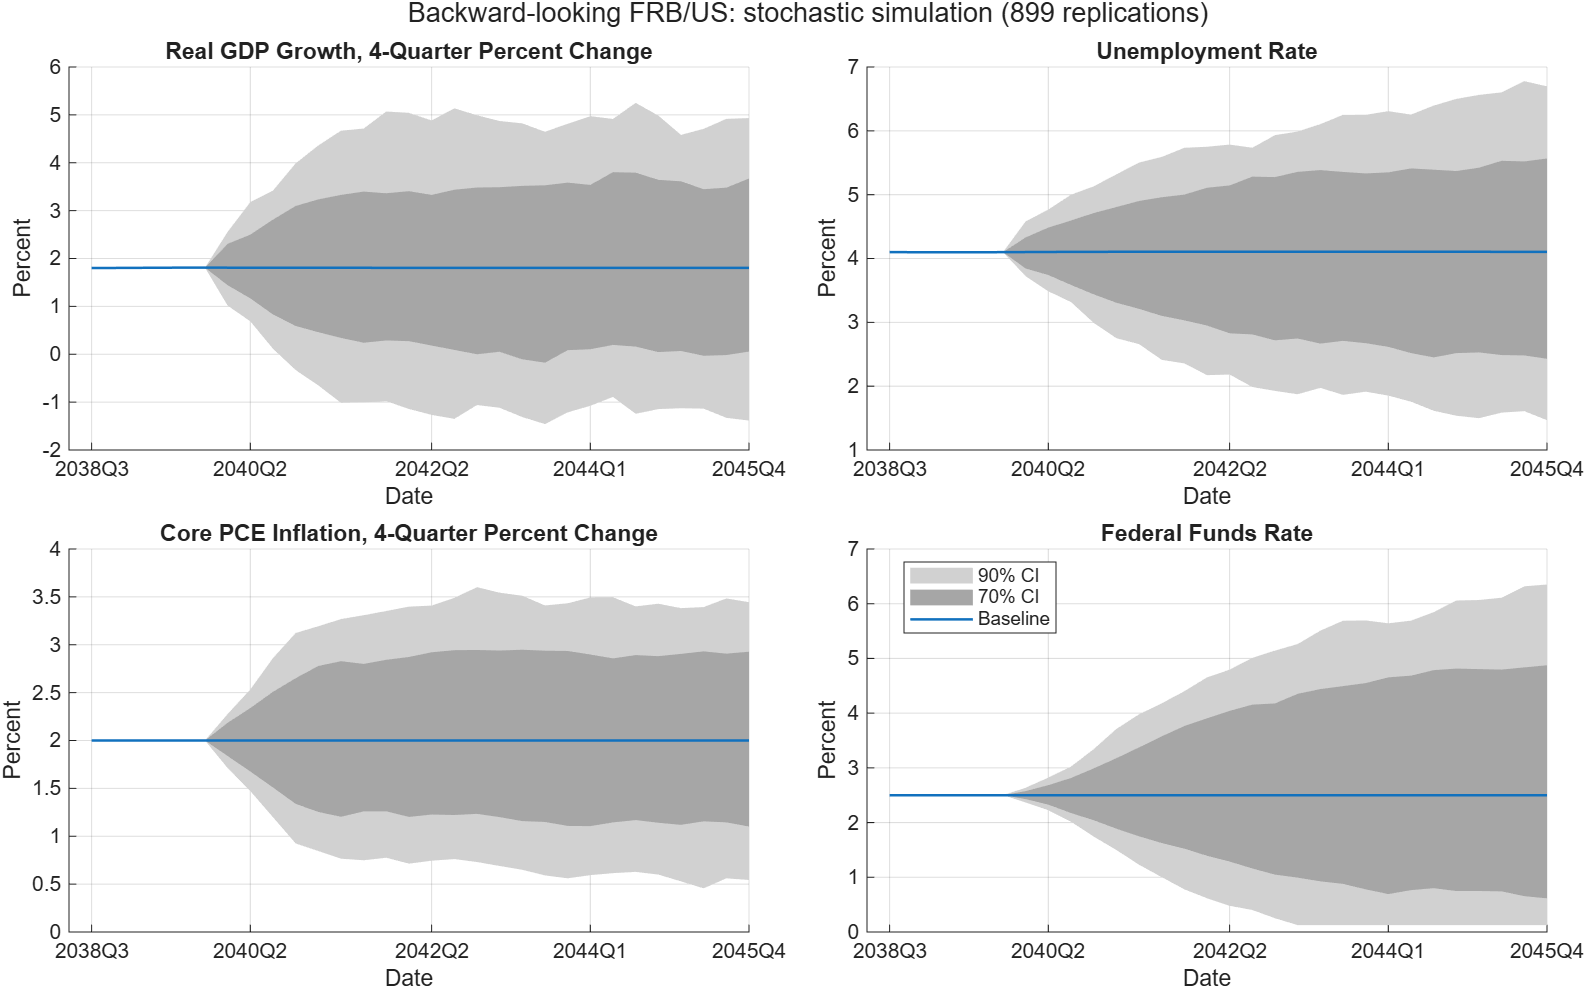
\includegraphics[width=0.94\linewidth]{stochastic_simulation_backward_pyfrbus_style.png}
\caption{Optional stochastic bootstrap output included with the v4 results.}
\label{fig:stochastic}
\end{figure}
\FloatBarrier

\section{Reproducibility and limitations}

The repository README gives commands for running MATLAB, regenerating the
translated files, running the Python tests, and compiling this report. Dynare
preprocessing creates model-specific packages under \texttt{dynare/}; those
generated directories are ignored by Git and are regenerated on demand.

The main limitations are the use of exact \texttt{max()} threshold equations,
the computational cost of repeated nonlinear solves, and the short terminal
horizon of the included MCE demonstration. The source equations and
coefficients are not re-estimated in this project. Any comparison with
BIMETS or pyfrbus should therefore distinguish model translation, data
calendar alignment, add-factor construction, solver tolerances, and charting
conventions.

\end{document}
